\section{Durchführung}
\label{sec:Durchfuehrung}
\subsection{Resonanzfrequenz}
\label{sec:Resonanzfrequenz}


\begin{figure}[h]
	\centering
	\label{fig:resonanzfrequenz}
		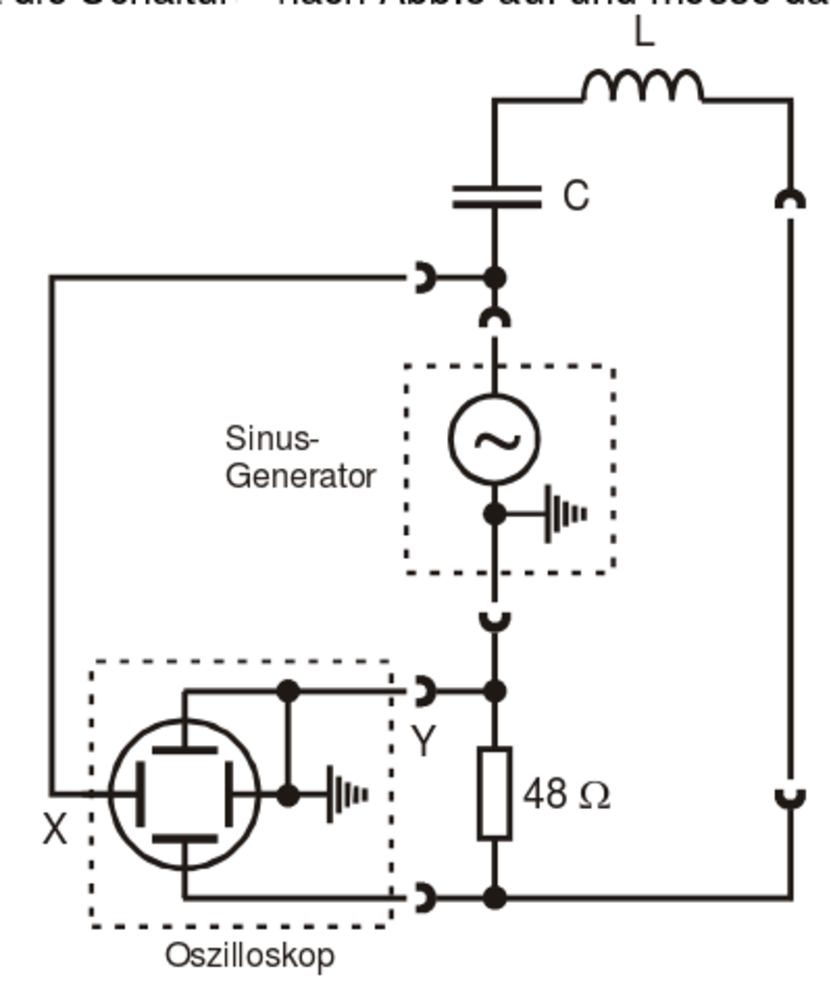
\includegraphics[width=0.5\textwidth]{Bilder/Resonanzfrequenz.pdf}
		\caption{Schaltung zur Bestimmung der Resonanzfrequenz.}
\end{figure}
Vor Messbeginn muss die fest eingestellte Resonanzfrequenz eines Schwingkreises gemessen und anschließend der andere darauf abgestimmt werden. Dazu wird die in Abbildung \ref{fig:resonanzfrequenz} gezeigte Schaltung aufgebaut. Für die grobe Messung der Frequenz wird der X-Eingang zunächst nicht benötigt. Der linke Schwingkreis wird durch den Frequenzgenerator zum Schwingen angeregt. Durch variieren der Frequenz am Generator ändert sich die am Widerstand $R_1$ abfallende Spannung $U_\mathup{R_1}(t)$. Die am Generator eingestellt Frequenz entspricht der Resonanzfrequenz $f_\mathup{res}$, wenn die Spannung $U_\mathup{R_1}(t)$ maximal wird.

Die Feineinstellung wird mit X-Eingang vorgenommen.
Dazu wird das Oszilloskop in XY-Betrieb umgeschaltet. Beiden Eingängen wird nun eine SPannung geliefert; die Widerstandsspannung $U_\mathup{R_1}(t)$ und die Erregerspannung $U(t)$ überlagern sich und werden gegeneinander aufgetragen. Auf dem Oszilloskop-Bildschirm wird diese Überlagerung als Lissajous-Figur sichtbar, nach derem Aussehen sich die Phasendifferenz zwischen Generator- und Schwingkreisstrom beurteilen lässt. 
Der Resonanzfall tritt ein, wenn für die Phasendifferenz $\Delta{\Phi}=0$  gilt und eine Gerade auf dem Bildschirm erscheint. Diese verläuft , wie in Abbildung LISSAJOUS zur Veranschaulichung dargestellt, im ersten und dritten Quadranten des Bildschirms.
Um den zweiten Schwingkreis auf dieselbe Frequenz zu eichen wird die Schaltung mit diesem Kreis erneut aufgebaut. Über eine variable Kapazität wird nach gleichem Verfahren der Resonanzfall eingestellt.

\subsection{Zeitabhängigkeit der Schwingungsenergie}

\begin{figure}[h]
	\centering
	\label{fig:versuchsaufbau}
		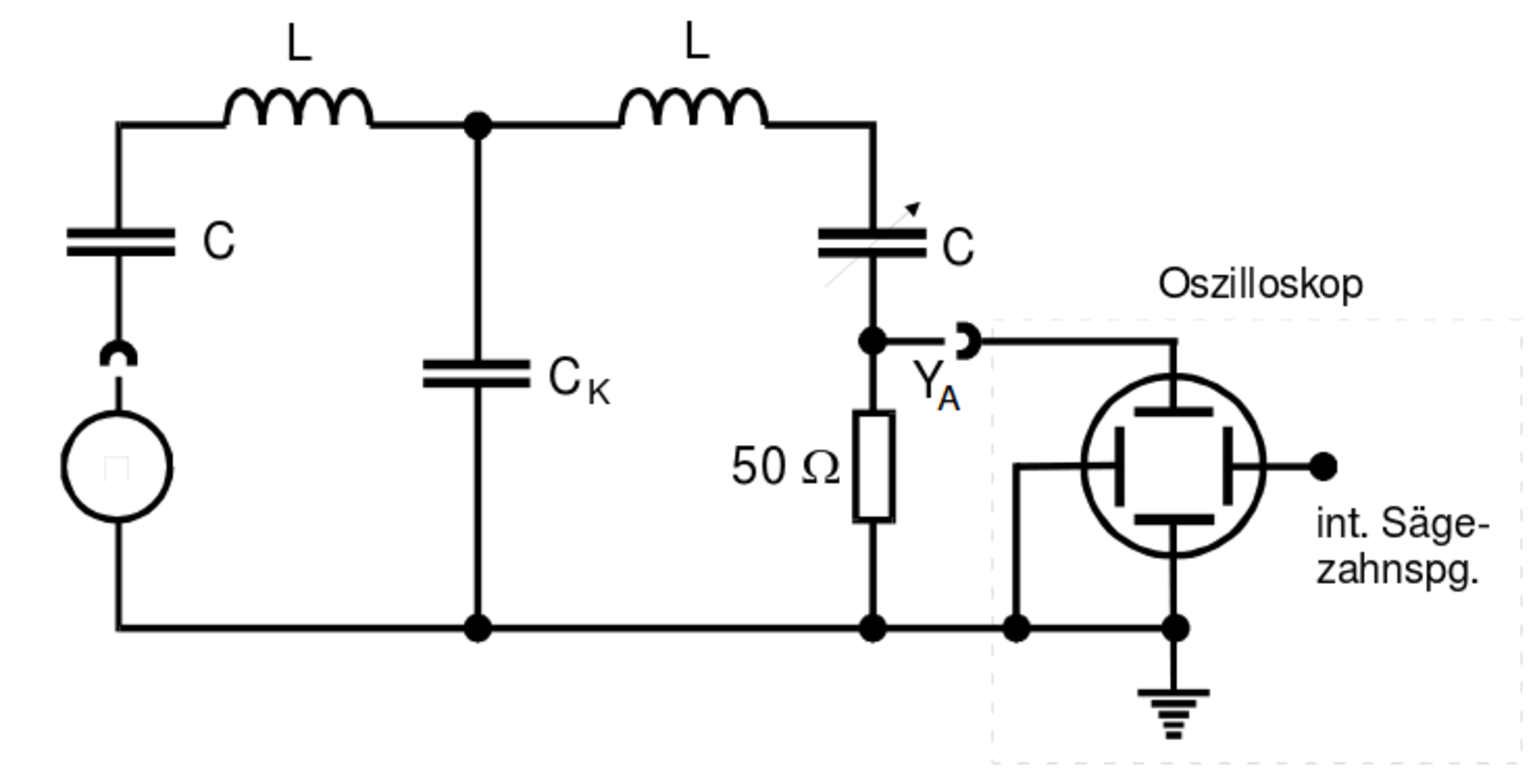
\includegraphics[width=0.5\textwidth]{Bilder/Versuchsaufbau.pdf}
		\caption{Schaltung zur Untersuchung gekoppelter Schwingkreise.}
\end{figure}
Für den ersten Versuchteil wird Schaltung 6 wie in Abbildung \ref{fig:versuchsaufbau} benötigt. Mit einem Rechteckimpuls wird ein Kreis zum Schwingen angeregt. Am ohmschen Widerstand fällt eine Spannung $U_\mathup{R_2}(t)$ ab, die durch das Oszilloskop dargestellt wird. Anschließend werden die Schwingungsmaxima pro Schwebungsperiode bei variablen Kopplungskapazitäten $C_\mathup{k}$ abgezählt.

\subsection{Frequenzen der Fundamentalschwingungen in Abhängigkeit der Koppelkapazität}
Der zweite Versuchsteil basiert auf derselben Schaltung, die Schwingung wird nun jedoch mit einem Sinusgenerator angeregt.
Die Kapazität $C_\mathup{k}$ wird erneut variiert. Für jede Kapazität wird die Lissajou-Figur betrachtet und die Frequenz so eingestellt, dass der Phasenunterschied $\Phi=0$ bzw. $\Phi=\pi$ beträgt. Bei $\Phi=0$ ergibt sich dieselbe Figur wie in Abschnitt \ref{sec:Resonanzfrequenz} erläutert; für $\Phi=\pi$  ergibt sich ebenfalls eine Gerade, die jedoch im zweiten und vierten Quadranten verläuft, also an der $U_\mathup{R_2}(t)$ gespiegelt ist.

\subsection{Frequenzabhängigkeit der Ströme}

Der dritte Versuchteil basiert, wie Teil 1 und 2, auf der Schaltung in Abbildung \ref{fig:versuchsaufbau}. Die Einstellungen des Generators werden so geändert, dass dieser in $20\cdot10⁻³\si\second$ ein Frequenzband von $10\cdot10⁻³-80\cdot10⁻³\,\si{\hertz}$ durchläuft. Dabei wird die am Widerstand abfallende Spannung $U_\mathup{R_2}(t)$ gegen die Zeit $t$ -- ein Maß für die Frequenz $f$ -- aufgetragen, sodass ein Spannungs-Frequenz-Diagramm entsteht, welches wie in Kapitel \ref{sec:erzwungen} beschrieben aussieht. Nun wird die Kopplungskapazität erneut variiert und die Zeitkoordinaten $t_+$ und $t_-$ der auftretenden Maxima notiert.
